\documentclass[12pt,a4paper,final]{article}
\usepackage[utf8]{inputenc}
\usepackage{amsmath}
\usepackage{amsfonts}
\usepackage{amssymb}
\usepackage{graphicx}
\usepackage{fancyhdr}
\usepackage{mathptmx}
\usepackage{float}
\usepackage{sectsty}
\usepackage[shortlabels]{enumitem}
\usepackage{array}
\sectionfont{\fontsize{12}{15}\selectfont}

\usepackage{etoolbox}
\makeatletter
\patchcmd{\l@section}
  {\hfil}
  {\leaders\hbox{\normalfont$\m@th\mkern \@dotsep mu\hbox{.}\mkern \@dotsep mu$}\hfill}
  {}{}
\makeatother
\usepackage[left=3.5cm,right=1.25cm,top=2.5cm,bottom=1.25cm]{geometry}
\graphicspath{ {Images/} }

\begin{document}
\newgeometry{left=1in,right=1in,top=1in,bottom=1in}
\section*{}
\pagenumbering{gobble}
\begin{center}
\Huge
\textbf{
Avoiding Road Traffic Congestion using Dynamic Traffic Assignment Approach
}

\vspace*{1.5cm}

\large
\textbf{
PROJECT SYNOPSIS
}

\vspace*{1.5cm}
\textbf{
BACHELOR OF ENGINEERING
}

\Large
\textbf{
Computer Engineering
}

\vspace*{1cm}
\large
SUBMITTED BY
\vspace*{1cm}
\linebreak
Adil Hussain
\linebreak
Mohammad Moheed Inamdar
\linebreak
Ajay Singh Rajpurohit
\linebreak
\linebreak
Under the guidance of
\linebreak
Mrs. Deepti Nirwal


\begin{figure}[h]
\begin{center}

\includegraphics[scale=1.0]{logo.png}
\end{center}
\end{figure}

\Large
\textbf{
Department of Computer Engineering
\linebreak
P. E. S. Modern College of Engineering,
\linebreak
Pune.
\linebreak
\linebreak
July 2017
}
\end{center}
\newpage

\tableofcontents
\listoffigures

\newgeometry{left=3.5cm,right=1.25cm,top=2.5cm,bottom=1.25cm}
\section{Title}
\setcounter{page}{1}
\pagenumbering{arabic}
\begin{flushleft}
\normalsize
Incremental Traffic Assignment Approach to avoid Road Traffic Congestion.
\linebreak

\noindent
\section{Domain}
Embedded Systems, Distributed Control Systems
\linebreak

\noindent
\section{Keywords}
Decentralized, Incremental Traffic Assignment, Greedy Algorithm, Web Service, IoT, Web Databases.
\linebreak
\linebreak
\noindent
\section{Team}
\begin{quotation}
Group Id: 4 \hfill
\linebreak

Team Members:
\begin{enumerate}
\item
Adil Hussain - 41024

\item
Mohammand Moheed Inamdar - 41025

\item
Ajay Singh Rajpurohit - 41061

\end{enumerate}
\end{quotation}

\noindent
\section{Objective}
\begin{enumerate}
\item
To Observe Current Traffic Conditions.
\item
To Mediate Road Traffic Flow.
\item
To Dynamically Control Traffic Signals.
\end{enumerate}

\noindent
\section{Scope}
\begin{enumerate}
\item
IoT Based Traffic Signal Control (Arduino)
\item
Decentralized Algorigthm to create changes in Signal timings
\end{enumerate}

\noindent
\section{Feasibility Study}
\begin{enumerate}
\item
Necessary Tools and their feasibility:\\
\begin{itemize}
\item Arduino Uno v3, low cost, feasible.\\
\item Internet GSM Connectivity, low cost, feasible.\\
\end{itemize} 
\item 
Schedule Feasibility\\
\begin{itemize}
\item Low number of modules.\\
\item Use of Simulation to speed up development.\\
\end{itemize}
\item 
Economic feasibility\\
\begin{itemize}
\item Commodity hardware.\\
\item Google Traffic API is free to use.\\
\item Redis DB is free to use.\\
\end{itemize}

\item 
Ethical Feasibility\\
\begin{itemize}
\item License applied to our project is GNU GPLv3.0\\
\item No copyrights or license laws were disobeyed.\\
\end{itemize}

\item 
Operational Feasibility\\
\begin{itemize}
\item Beneficial as it uses Least Modification to current Traffic System.\\
\item Doesn't inhibit driver's experience.\\
\item Reduces chances of Congestion Creation by preventing it from building up.\\
\end{itemize}
\end{enumerate}

\noindent
\section{Technical Details}
\begin{quotation}
\textbf{Platform}
\begin{itemize}

\item
Linux for Arduino

\end{itemize}

\textbf{Software Specification}
\begin{itemize}

\item
Python 2.7+, 3.5+

\end{itemize}

\textbf{Hardware Specification}
\begin{itemize}
\item
Arduino Uno
\end{itemize}

\textbf{Dataset}
\begin{itemize}
\item
LatLong Objects from Google Traffic API
\end{itemize}
\end{quotation}

\noindent
\section{Innovativeness and Usefulness}
\begin{enumerate}
\item
Implementation of an Automatic Solution to Traffic Assignment Problem
\item
Dynamic / Self-Optimizing Solution
\item
Deployable over any existent Traffic Systems
\end{enumerate}

\noindent
%%\section{Market Potential and Competitive Advantage}
%%\begin{enumerate}
%%\item
%%Market Potential and Competitive Advantage 1	% No need to change existing Infrastructure
%%\item
%%Market Potential and Competitive Advantage 2	% about Rs. 1000/- maximum investment per Signal
%%\item
%%Market Potential and Competitive Advantage 3	% Ready to deploy system, easy to setup and work with.

%%\end{enumerate}

\noindent
\pagebreak
\section{Brief Description}
\begin{figure}[H]
\begin{center}
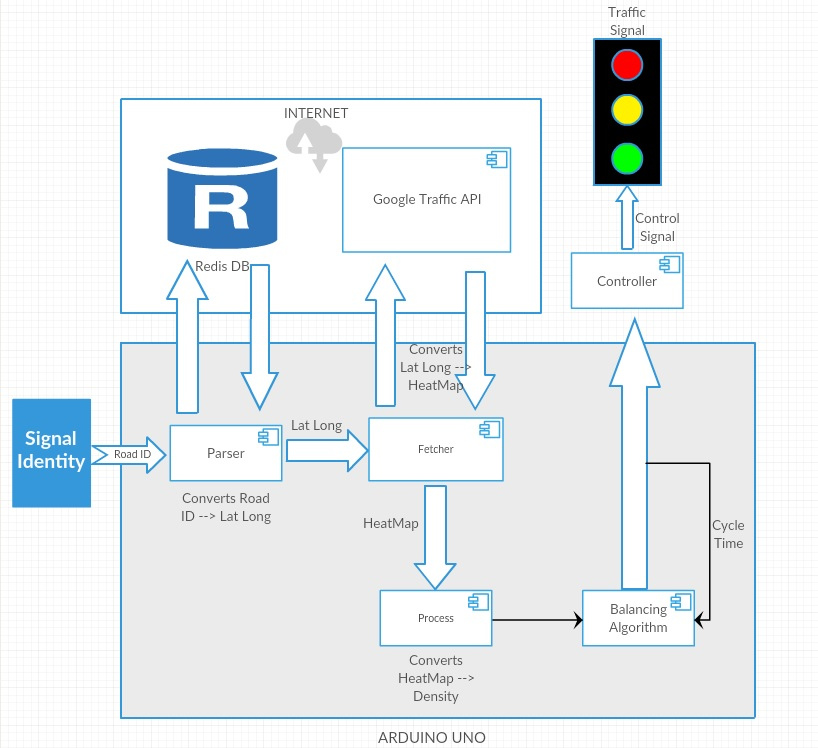
\includegraphics[scale=0.5]{architecture.jpg}
\caption{System Architecture Diagram}
\end{center}
\end{figure}

%\begin{figure}[H]
%\begin{center}
%\includegraphics[scale=0.5]{Architecture-2.png}
%\caption{Architecture Diagram}
%\end{center}
%\end{figure}

\begin{enumerate}
\item
Road ID: The roads connected to the current signal
\item
LatLong Objects: Objects defined via Google Traffic API. Contains Coordinates of point locations to consider (road).
\item
HeatMap: The density map of traffic with respect to a colour gradient.
\item
Cycle Time: The duration of Red, Green and Yellow lights for each lane as a Set.
\end{enumerate}

\newpage
\noindent

\section{Probable Deadline for project completion}
Last week of March - 2018

%\section{Major Milestones and Dates}
%22^{nd} August 2017 - Topic Finalization
%23^{rd} September 2017 - 1st Revision of Topic (rethink)

\section{References}

\begin{enumerate}[label={[\arabic*]}]
\item Alain Kibangou, et. al., “An Integrated and Scalable Platform for
 Proactive Event-Driven Traffic Management,” \textit{Arxiv.org}, 8th March 2017.

\item Carlos Gershenso, “Self-Organizing Traffic Lights,” \textit{Arxiv.org},
 5th Feb 2008.

\item Moshe E. Ben-Akiva, et. al., “A dynamic traffic assignment model
 for highly congested urban networks,” \textit{Elsevier}, 6th Feb 2012.

\item Pu Wang, et. al., “Understanding Road Usage Patterns in Urban
 Area,” \textit{SCIENTIFIC REPORTS}, vol 2, no. 1001, 20 December 2012.

\item Nasrin Taherkhani and Samuel Pierre, “Centralized and Localized
 Data Congestion Control Strategy for Vehicular Ad Hoc Networks Using
 a Machine Learning Clustering Algorithm,” \textit{IEEE TRANSACTIONS ON
 INTELLIGENT TRANSPORTATION SYSTEMS}, March 20, 2016.

\end{enumerate}
\end{flushleft}
\end{document}

